% The figures' text fixture (tests/fixtures/pdf/figures/README.md): one page of vector figures whose text the engine cuts into
% figure units, in each shape the content class `figures` meets. Ours, CC0. Made by scripts/make-figure-fixture.mjs, which
% writes the layout compile's points before \documentclass (marks.mjs POINTS_TEX) and compiles it in the pinned TeX Live.
\documentclass{article}
\usepackage[margin=2cm]{geometry}
\usepackage{graphicx}
\usepackage{pgfplots}
\pgfplotsset{compat=1.18}
\pagestyle{empty}
\begin{document}
\noindent
% (a) a pgfplots axis: its title, its x label, its y label turned (a rotated label), and a legend of four entries close
% together (a dense legend)
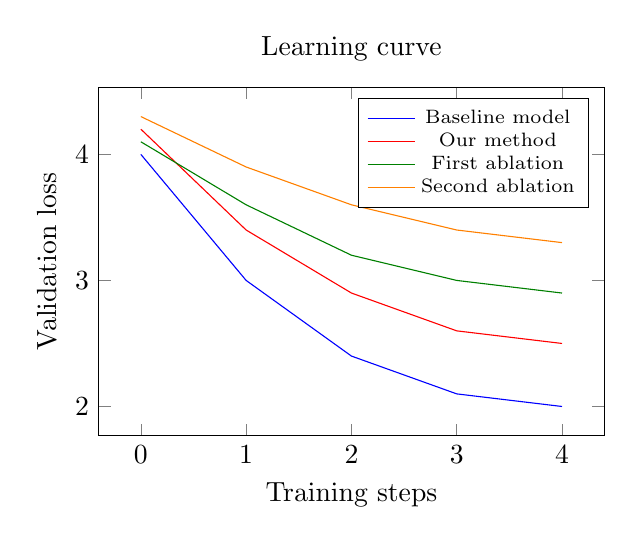
\begin{tikzpicture}
\begin{axis}[width=8cm, height=6cm, title={Learning curve}, xlabel={Training steps}, ylabel={Validation loss},
  legend style={at={(0.97,0.97)}, anchor=north east, font=\scriptsize, row sep=-2pt}]
\addplot[blue] coordinates {(0,4) (1,3) (2,2.4) (3,2.1) (4,2)};
\addplot[red] coordinates {(0,4.2) (1,3.4) (2,2.9) (3,2.6) (4,2.5)};
\addplot[green!50!black] coordinates {(0,4.1) (1,3.6) (2,3.2) (3,3) (4,2.9)};
\addplot[orange] coordinates {(0,4.3) (1,3.9) (2,3.6) (3,3.4) (4,3.3)};
\legend{Baseline model, Our method, First ablation, Second ablation}
\end{axis}
\end{tikzpicture}\hfill
% (b) a TikZ diagram: a node's text in a box, and a label beside an arrow
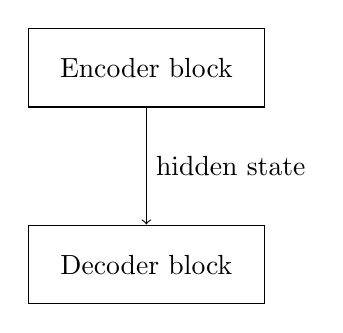
\begin{tikzpicture}
\node[draw, minimum width=3cm, minimum height=1cm] (e) at (0,0) {Encoder block};
\node[draw, minimum width=3cm, minimum height=1cm] (d) at (0,-2.5) {Decoder block};
\draw[->] (e) -- node[right] {hidden state} (d);
\end{tikzpicture}

\vspace{1cm}\noindent
% (c) an included PDF whose fonts carry a /ToUnicode; (d) one whose font gives a code, not a character, for each glyph
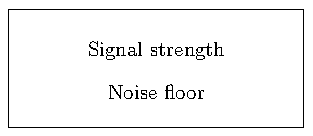
\includegraphics{inc-tounicode.pdf}\hfill
\includegraphics{inc-codes.pdf}
\end{document}
